\chapter{Deep Learning}
\label{cp:dp}
This chapter consists of four sections. 
\begin{itemize}
    \item \textbf{Section} \ref{dpintro}, a brief introduction to deep learning neural networks, including its history, development and current application.
    \item \textbf{Section} \ref{cnn}, decribing details of about Convolutional Neural Networks, including different types of layers and their functionas.
    \item \textbf{Section} \ref{training}, talking about the techqiues used in deep learning training process, which make training get convagence faster and more accurate.  
\end{itemize} 

\section{Introduction}
    \label{dpintro}
    As a subdiscipline of machine learning, deep learning attempts to perform data abstraction at high level hvia multiple processing layers. It is an algorithm based on the data representation learning of machine learning. Observations (e.g., an image) can appear in various forms, such as a vector of specific pixel intensity, or more abstractly, a series of edges, regions of certain shape, etc. Learning tasks can be completed more easily by applyingg some special representation methods (for example, facial recognition or facial expression recognition). The merit of deep learning lies in transforming manual acquisition into unsupervised or semi-supervised learning along with its efficient algorithms of hierarchical feature extraction \cite{schmidhuber2015deep}.
    %Deep learning is a branch of machine learning, which attempts to use high-level abstraction of data with multiple processing layers. Deep learning is an algorithm based on the representation learning of data in machine learning. Observations (e.g., an image) can be represented in a variety of ways, such as a vector of each pixel intensity value, or more abstractly represented as a series of edges, regions of a particular shape, and the like. It is easier to learn tasks from instances using some specific representation methods (for example, face recognition or facial expression recognition). The advantage of deep learning is to replace the manual acquisition feature with unsupervised or semi-supervised feature learning and hierarchical feature extraction efficient algorithms . \\

    Previous works on deep learning (or Cybernetics as called at that time) were first published during 1940s to 1960s, which discusses biologically inspired models like Perceptron, Adaline, or Multi Mayer Perceptron \cite{rosenblatt2000probabilistic, schmidhuber2015deep}. Then, from 1960s to 1980s backpropagation was invented and the second wave named Connectionism followed up \ cite {rumelhart1986learning}sn. This algorithm has been active up to now and is currently utilized for optimization of Deep Neural Networks. Convolutional Neural Networks (CNNs) is among the most outstanding contributions, which is designed to identify visual patterns of relative simplicity, such as handwritten characters \cite{lecun1995convolutional}. Finally, the appearance of more complex architectures in 2006 marks the arrival of deep learning’s modern era\cite{hinton2006fast,bengio2007greedy,huang2007unsupervised}. Breakthroughs in processing of speech and natural language (2011) as well as image classification at ILSVRC\footnote{\url{http://www.image-net.org/challenges/LSVRC/}} the scientific competition (2012) have made deep learning a conqueror in many Machine Learning communities like Reddit and winner of challenges beyond conventional applications\footnote{\url{http://blog.kaggle.com/2014/04/18/winning-the-galaxy-challenge-with-convnets}}. \\


    %Early works on Deep Learning, or rather on Cybernetics, was made in $1940$-$1960$s, and describe biologically inspired models such as the Perceptron\cite{rosenblatt2000probabilistic,schmidhuber2015deep}. Then, a second wave called Connectionism came in the $1960$s-$1980$s with the invention of backpropagation \cite{rumelhart1986learning}, which has become the algorithm of choice to optimize Deep Neural Networks(DNNs). A notable contribution is the Convolutional Neural Networks (CNNs) designed, at this time, to recognize relatively simple visual patterns, such as handwritten characters \cite{lecun1995convolutional}. Finally, the modern era of Deep Learning has started in 2006 with the creation of more complex architectures \cite{hinton2006fast,bengio2007greedy,huang2007unsupervised}. Since a breakthrough in speech and natural language processing in 2011, and also in image classification during the scientific competition ILSVRC in 2012, Deep Learning has conquered many Machine Learning communities, such as Reddit, and won challenges beyond their conventional applications area \footnote{\url{http://blog.kaggle.com/2014/04/18/winning-the-galaxy-challenge-with-convnets}}. \\

    %Early works on deep learning, or rather earlier works that were once called "cybernetics", were produced in the 1940s - 1960s and described biologically inspired models such as Perceptron, Adaline or Multi Mayer Perceptron. \cite{rosenblatt2000probabilistic, schmidhuber2015deep }. Then, in the 1960s and 1980s, a second wave of backpropagation occurred, inventing the back propagation \cite{rumelhart1986learning}. The algorithm continues to the present and is currently the preferred algorithm for optimizing deep neural networks. One notable contribution is convolutional neural networks (CNNs), which are currently designed to identify relatively simple visual patterns, such as the handwritten character \cite{lecun1995convolutional}. Finally, the modern era of deep learning began in 2006, creating a more complex architecture \cite{hinton2006fast, bengio2007greedy, huang2007unsupervised}. Since breakthroughs in voice and natural language processing in 2011 and image classification during the 2012 ILSVRC Science Competition, deep learning has conquered many machine learning communities, such as Reddit, and has won challenges beyond its traditional application areas\footnote{\url{http://blog.kaggle.com/2014/04/18/winning-the-galaxy-challenge-with-convnets}}. \\

    Especially, deep learning has enormously impacted the field of computer vision by achieving unprecedented performance on tasks of image classification, objects detection, image segmentation, image captioning and so on in the past four years \cite{DBLP:journals/corr/GuWKMSSLWW15}. Such huge progress is primarily built up on the enlargement  in computational resources such as frameworks (e.g.s TensorFlow\footnote{\url{https://www.tensorflow.org/}}), modern GPU implementations (e.g.  Cudnn\footnote{\url{https://developer.nvidia.com/cudnn}}), increasing amount of available annotated data, and participation in open source codes and share models based on community. Thanks to these advances, morer audience are accessible to the expertise that is necessary for the training of modern convolutional networks. Higher accuracy can be achieved through training of larger and deeper architectures on greater datasets every year, while phenomenal outcomes have been exhibited by the  already trained ones when they are transferred to smaller datasets or evaluated with varied visual tasks. \\

    %Especially during the last four years, Deep Learning has made a tremendous impact in computer vision reaching previously unattainable performance on many tasks such as image classification, objects detection, image segmentation or image captioning \cite{DBLP:journals/corr/GuWKMSSLWW15}. This progress have been made possible by the increase in computational resources, thanks to frameworks such as TensorFlow\footnote{\url{https://www.tensorflow.org/}}, modern GPUs implementations such as Cudnn\footnote{\url{https://developer.nvidia.com/cudnn}}, the increase in available annotated data, and the community-based involvement to open source codes and to share models. These facts allowed for a much larger audience to acquire the expertise needed to train modern convolutional networks. Thus, larger and deeper architectures are trained on bigger datasets to achieve better accuracy each year. Also, already trained models have shown astonishing results when transfered on smaller datasets and evaluated on different visual tasks. \\

    %With deep learning becoming more and more popular in many fields of researching, some classical methods can be replaced by deep learning. Many successful application of deep learning can be found in computer vision part, like image segmentation\cite{lecun2015deep},objection recognition\cite{he2016deep}.
    The increasing popularity of deep learning in various research fields enables it the replacement of some conventional approachesg. The computer vision section gives many successful applications, such as image segmentation\cite{lecun2015deep},objection recognition\cite{he2016deep}.
     \begin{figure}[!ht]
        \centering
        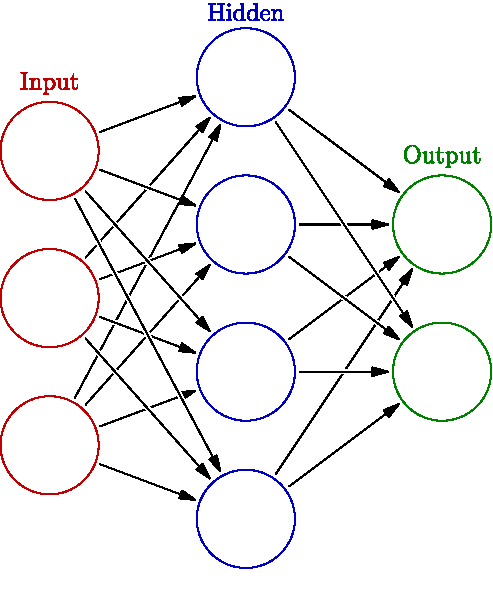
\includegraphics[scale = 0.5]{Figures/Colored_neural_network}
        \caption{visulization of one simple $3$-layers neural networks, including input layer, hidden layer and output layer, \textit{retrieved from Wikipedia}}
    \end{figure}

\section{Convolutional Neural Networks}
    \label{cnn}
    An input layer, an output layer, and multiple hidden layers make up the complete convolutional neural network. Normally, the hidden layers include convolutional layer, pooling layers, fully connected layers, and normalization layers. \\

    The process in neural networks is described classically as a convolution, while it is a cross-correlation rather than a convolution in terms of math. Only indices in the matrices are meaningful, which are thus assigned with weights. 

    \subsection{Convolutions}
    An effective solution to such issue by utilizing the structure of image-encoded information is to assume that compared with the pixels at the opposite corners of the image, the spatially closer ones can construct some certain feature of interest cooperatively. Further, an important (smaller) feature in image label definition tends to possess equal importance wherever it is within the image. \\
    %It turns out that there is a very efficient way of pulling this off, and it makes advantage of the structure of the information encoded within an image – it is assumed that pixels that are spatially closer together will ``cooperate'' on forming a particular feature of interest much more than ones on opposite corners of the image. Also, if a particular (smaller) feature is found to be of great importance when defining an image's label, it will be equally important if this feature was found anywhere within the image, regardless of location. \\

    A convolution operator is entered. For a given two-dimensional image, I, and a small matrix, $\pmb{K}$ with size $h \times w$, (known as a convolution kernel), which is presumptively encoded with an extraction way of an interesting image feature, the convolved image, $\pmb{I} * \pmb{K}$, is computed by overlaying the kernel on image top  in every possible way and recording the sum of elementwise products between the image and the kernel:
    %Enter the convolution operator. Given a two-dimensional image, I, and a small matrix, $\pmb{K}$ of size $h \times w$, (known as a convolution kernel), which we assume encodes a way of extracting an interesting image feature, we compute the convolved image, $\pmb{I} * \pmb{K}$ , by overlaying the kernel on top of the image in all possible ways, and recording the sum of elementwise products between the image and the kernel:

    \begin{equation}
        (\pmb{I} * \pmb{K})_{xy} = \sum_{i=1}^{h}\sum_{j=1}^{w} \pmb{K}_{ij}\cdot \pmb{I}_{x+i-1, y+j-1}
    \end{equation}

    \begin{figure}[!h]
        \centering
        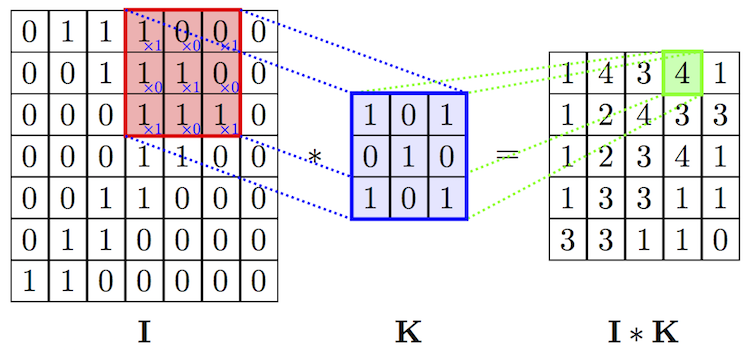
\includegraphics[scale=1.3]{Figures/convolve.png}
        \caption{One simple example of convolution.}
        \label{con}
    \end{figure}

    \subsection{Convolutional layers}
    Normal RGB images are represented by matrices containing color information in the form of Red-Gray-Blue color codes. An image therefore has size $h\times w \times d$, where $d$ is the number of channel of image, in normal RGB images, $d=3$. However, in the case of this thesis, channels consist of $[m, v_x, v_y, \omega, n_x]$, therefore in its case, $d=5$. Convolutional layers are essential layers in CNNs, producing feature maps from input images or lower level feature maps. \\

    Convolutional layers includes a kernel (or filter). Let $K$ be a kernel with $x$ rows, $y$ columns and depth $d$. Then the kernel with size ($K_x \times K_y \times d$) works on a receptive field ($K_x \times K_Y$) on the image. The kernel height and width are smaller than the input image height and width. The kernel slides over (convolves with) the image, producing an feature map (Figure \ref{con}). Convolution is the sum of the element-wise multiplication of the kernel and the original image. Note that the depth d of the kernel is equal to the depth of its input. Therefore, it varies within the network. Usually the depth of an image is the number of color channels, the three RGB channels. In this case, $d=5$. \\

    The kernel stride is a free parameter in convolutional layers which has to be defined before training. The stride is the number of pixels by which the kernel shifts at a time. A drawback of using convolutional layers is that it decreases the output map size. A larger stride will result in a smaller sized output. Equations \ref{out} show the relationship between output size $O$ and input size of an image $I$ after convolution with stride $s$ and kernel $K$. Furthermore, the feature map size decreases as the number of convolutional layers increases. Row output size $O_x$ and column output size $O_y$ of convolutional layers are determined as follows:
    \begin{equation}
        \begin{cases}
            O_x = \frac{I_x-K_x}{s} + 1 \\
            O_y = \frac{I_y - K_Y}{s} + 1 \\
        \end{cases}
        \label{out}
    \end{equation}
    As an example, an image of size ($32\times 32 \times 3$), a kernel of size ($3\times 3\times 3$) and a stride $s=1$ result in an activation map of size ($30 \times 30 \times 1$). Using additional $n$ kernels, the activation map becomes ($30\times30\times n$). So, additional kernels will increase the depth of the convolutional layer output. Online resources can be referred to for more animation examples with different types of convolution\footnote{\url{https://github.com/vdumoulin/conv_arithmetic}}.\\

    \begin{figure}[!h]
        \centering
        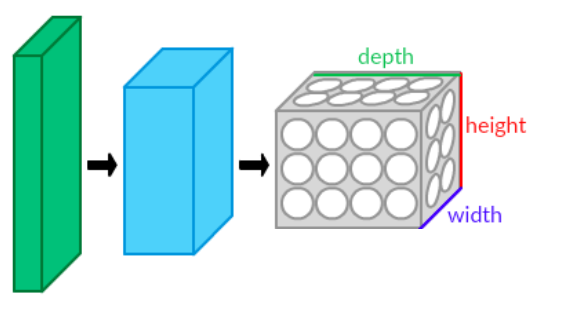
\includegraphics[scale = 0.3]{Figures/Conv_layers.png}
        \caption{Visualization of convolutions network, \textit{retrieved from Wikipedia}}
    \end{figure}

    \subsection{Activation Layer}
    Essentially, whether a neuron should be activated is decided by the activation functions. As a feature for the artificial neural networks of prime importance, they are in charge of distinguishing the relevant signals received by neuron from the irrelevant ones. Normally, we can express the general function as Equation \ref{ac}. And one mathematical model is shown in Figure \ref{action} to describe how activation function is.

    \begin{equation}
        y = f_{Activation}(\sum_{i}(w_i \cdot x_i) + bias)
        \label{ac}
    \end{equation}

    \begin{figure}
        \centering
        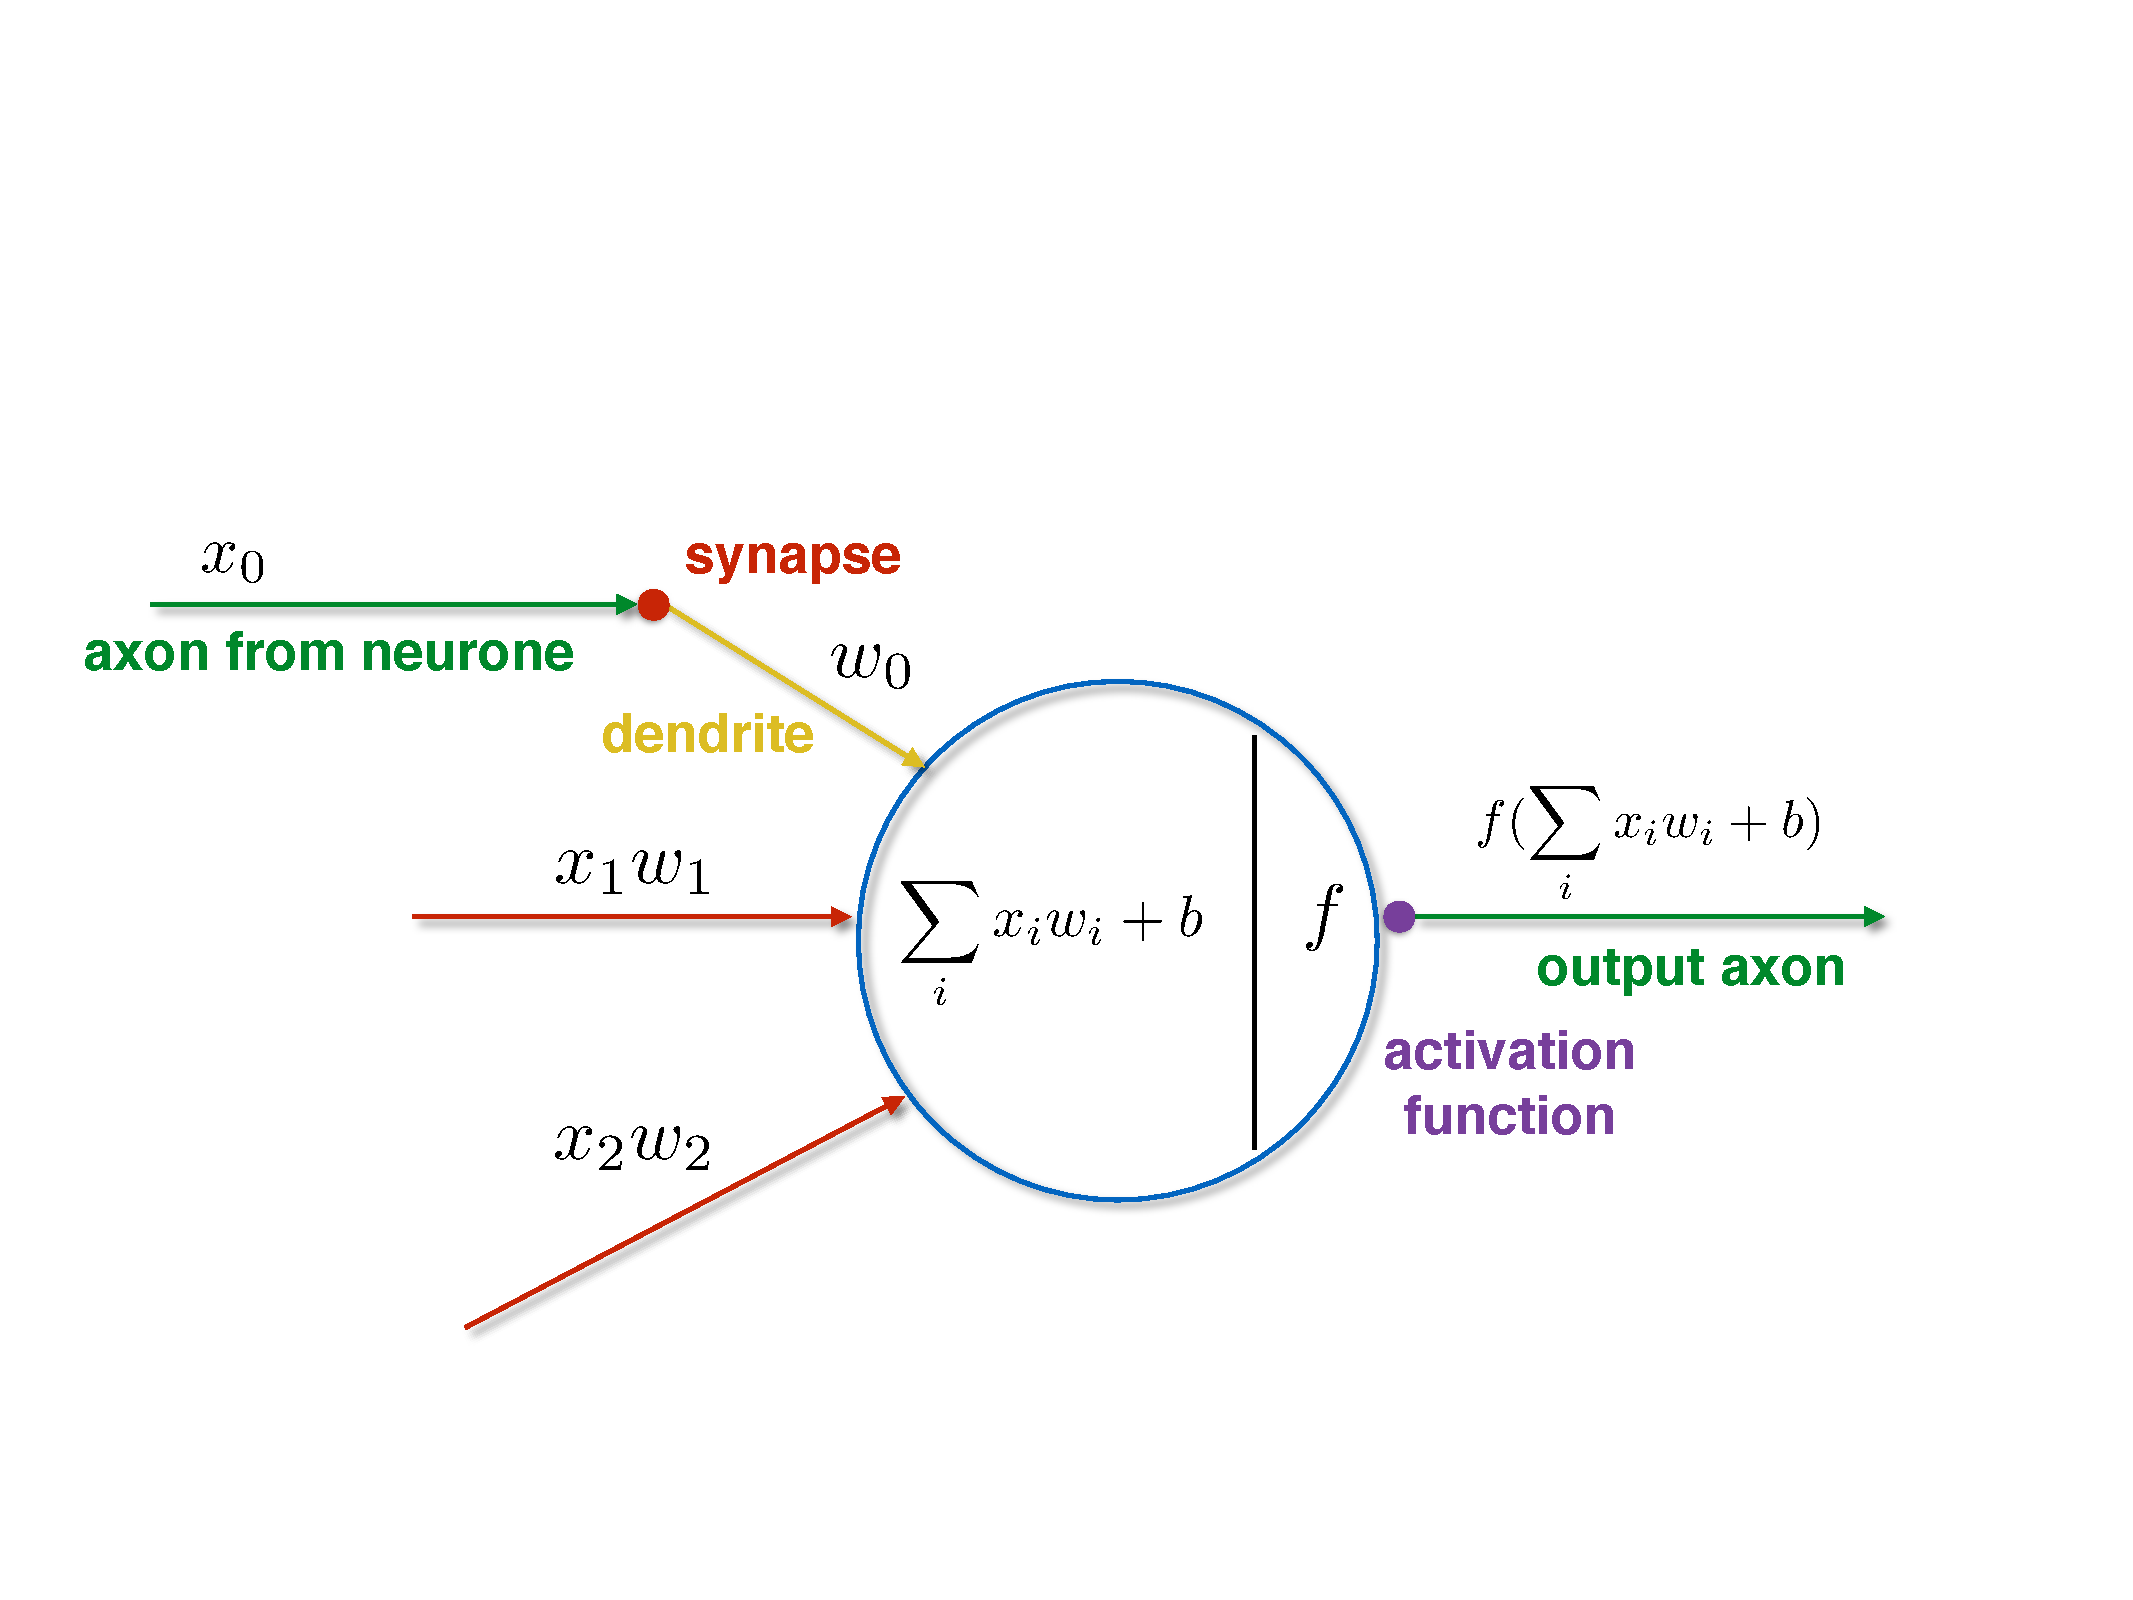
\includegraphics[scale=0.3]{Figures/action.pdf}
        \caption{Mathematical model for describing activation function}
        \label{action}
    \end{figure}

    By transforming the input signal, the nonlinear activation function can be obtained, which, in turn,  is subsequently sent to the next layer of neurons as an input. Rectified Linear Unit (ReLU) is considered as the activation function that enjoys the most pervasive application nowadays. More details are presented below. 

    \subsubsection{Rectified Linear Unit}
    ReLU commonly appears in the mathematical form as follows,
    \begin{equation}
        y = max(0, x)
    \end{equation}
    Thanks to its linear non-saturating form (e.g. a factor of 6 in \cite{krizhevsky2012imagenet}), a great accelerating effect on converging the stochastic gradient descent was discovered for ReLU when compared with the $sigmoid$/$tanh$ functions. Since then, it has become a very favorable approach. Vanishing or exploding gradient can hardly affect it actually. Further, it is much more economical than the conventional s  exponentials. Nonetheless, ReLU cannot cater for all datasets and architectures, for it may get rid of every piece of negative information.

    \subsection{Pooling Layer}
    Pooling layers are also known as downsampling layers. A commonly used pooling is maxpooling (figure \ref{maxpooling}). The downsampled output is produced by taking the maximum input value within the kernel, resulting in the output with a decreased size. There are several other methods which are commonly used in neural networks, such as average pooling and L2-norm pooling. Average pooling used to be a common method, while it is quitting the historical arena these days due to the more practical mmaxpooling\cite{scherer2010evaluation}.\\

    There are two important arguments for implementinf pooling layers,
    \begin{enumerate}
        \item Decreasing the number of weights.
        \item Decreasing the chance of overfitting the training data.
    \end{enumerate}
    \begin{figure}[!h]
        \centering
        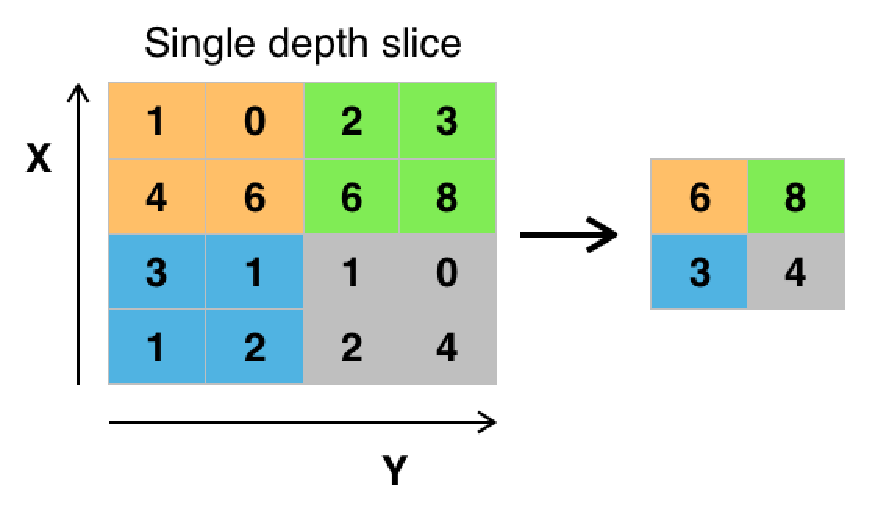
\includegraphics[scale=0.5]{Figures/Max_pooling.pdf}
        \caption{Maxpooling with a ($2\times 2$) kernel and stride $s=2$. Maxpooling layers reduce spatial dimension of the input \cite{li2015convolutional}}
        \label{maxpooling}
    \end{figure}

    \subsection{Fully Connected Layer}
    Following the steps of convolutional and maxpooling layers, fully connected layer realizes the high-level reasoning in neural networks eventually. .As what a regular neural network shows, all activations in the above-mentioned layers are connected by the neurons at a fully connected layer. A matrix multiplication and the follow-up bias offset will then complete all the calculations of these activations.

    \subsection{Batch Normalization}
    \label{batchnor}
    Because of its assistance in faster convergence, this layer shoots to popularity rapidlyr\cite{ioffe2015batch}. By adding  a normalization step of shifting inputs to zero-mean and unit variance, it achieves the comparability across features of inputs in every trainable layers. Consequently, a high learning rate is guaranteed during the network learning process. \\

    Besides, activation functions like TanH and Sigmoid are protected by it from getting stuck in saturation mode (e.g. gradient equal to $0$).

    \section{Training Method}
    \label{training}
    \subsection{Loss Function}
    The value of the loss function $L$ represents the difference between the training image after it has propagated through the network and desired annotated output image.\\ 

    Two assumptions are made about this loss function. 
    \begin{enumerate}
        \item It be able to be defined as the average over the loss functions for individual training images, as the training often is carried out in batches.
        \item It should be able to be defined as a function of the network outputs. 
    \end{enumerate}

    Below a brief overview is given of some widely used loss functions, where $f_{\theta}(x_i)$ are the neuron outputs and $y_i$ are the desired outputs.
    \subsubsection{Quadratic Cost Function}
    The Mean Squared Error (MSE) cost function is one of the simplest cost functions. Normally it will be used in estimation problems\cite{boureau2008sparse}.
    \begin{equation}
        L =\frac{1}{N}\sum_{n=1}^{N}(f_{\theta}(x_i) - y_i)^2
        \label{eq:mse}
    \end{equation}


    \subsection{Overfitting}
    OOverfitting is a problem that arises in neural network training. When a model is overfitted to the training data, it loses its capability of generalization. The model has learned the training data, including noise, in such a great extent that it has failed to capture underlying general information. CNNs have a large number of weights to be trained, therefore overfitting can occur due to training too few training examples.

    \subsubsection{Regularization L2}
     As the first primary route to averting overfitting, the classical method of weight decay increased one more term to the cost function as a penalization for parameters in each dimension, so that the network is prevented from exact modelling of the training data and generalization of new examples is thus ensured. 

    \begin{equation}
        Error(x, y) =  Loss(x, y) + \sum_{i}\theta_i
    \end{equation}
    where $\theta$ is with a vector containing all parameters in the network.

    \subsubsection{Data augmentation}
    The size of the training set can be enlarged by data augmentation in order to prohibit memorizing of the whole set by the model. A few types may be involved depending on the dataset. For instance, objects  supposed to be constantly rotating,  such as galaxies or planktons, will fiti different kinds of rotations to the original images.

    \subsubsection{Dropout}
    Dropout layers\cite{srivastava2014dropout} are a tool to prevent overfitting (Figure \ref{dropout}). In dropout, nodes and its connections are randomly dropped from the network. Dropout constrains the network adaptation to the training set, consequently it prevents that the weights are not too much fitted this data. Training data will thus have reduced performance difference with validation date. Dropout layers are used during training only, not during validation or testing. Nowadays, dropout method has been the main method to prevent overfitting.

    \begin{figure}[!h]
        \centering
        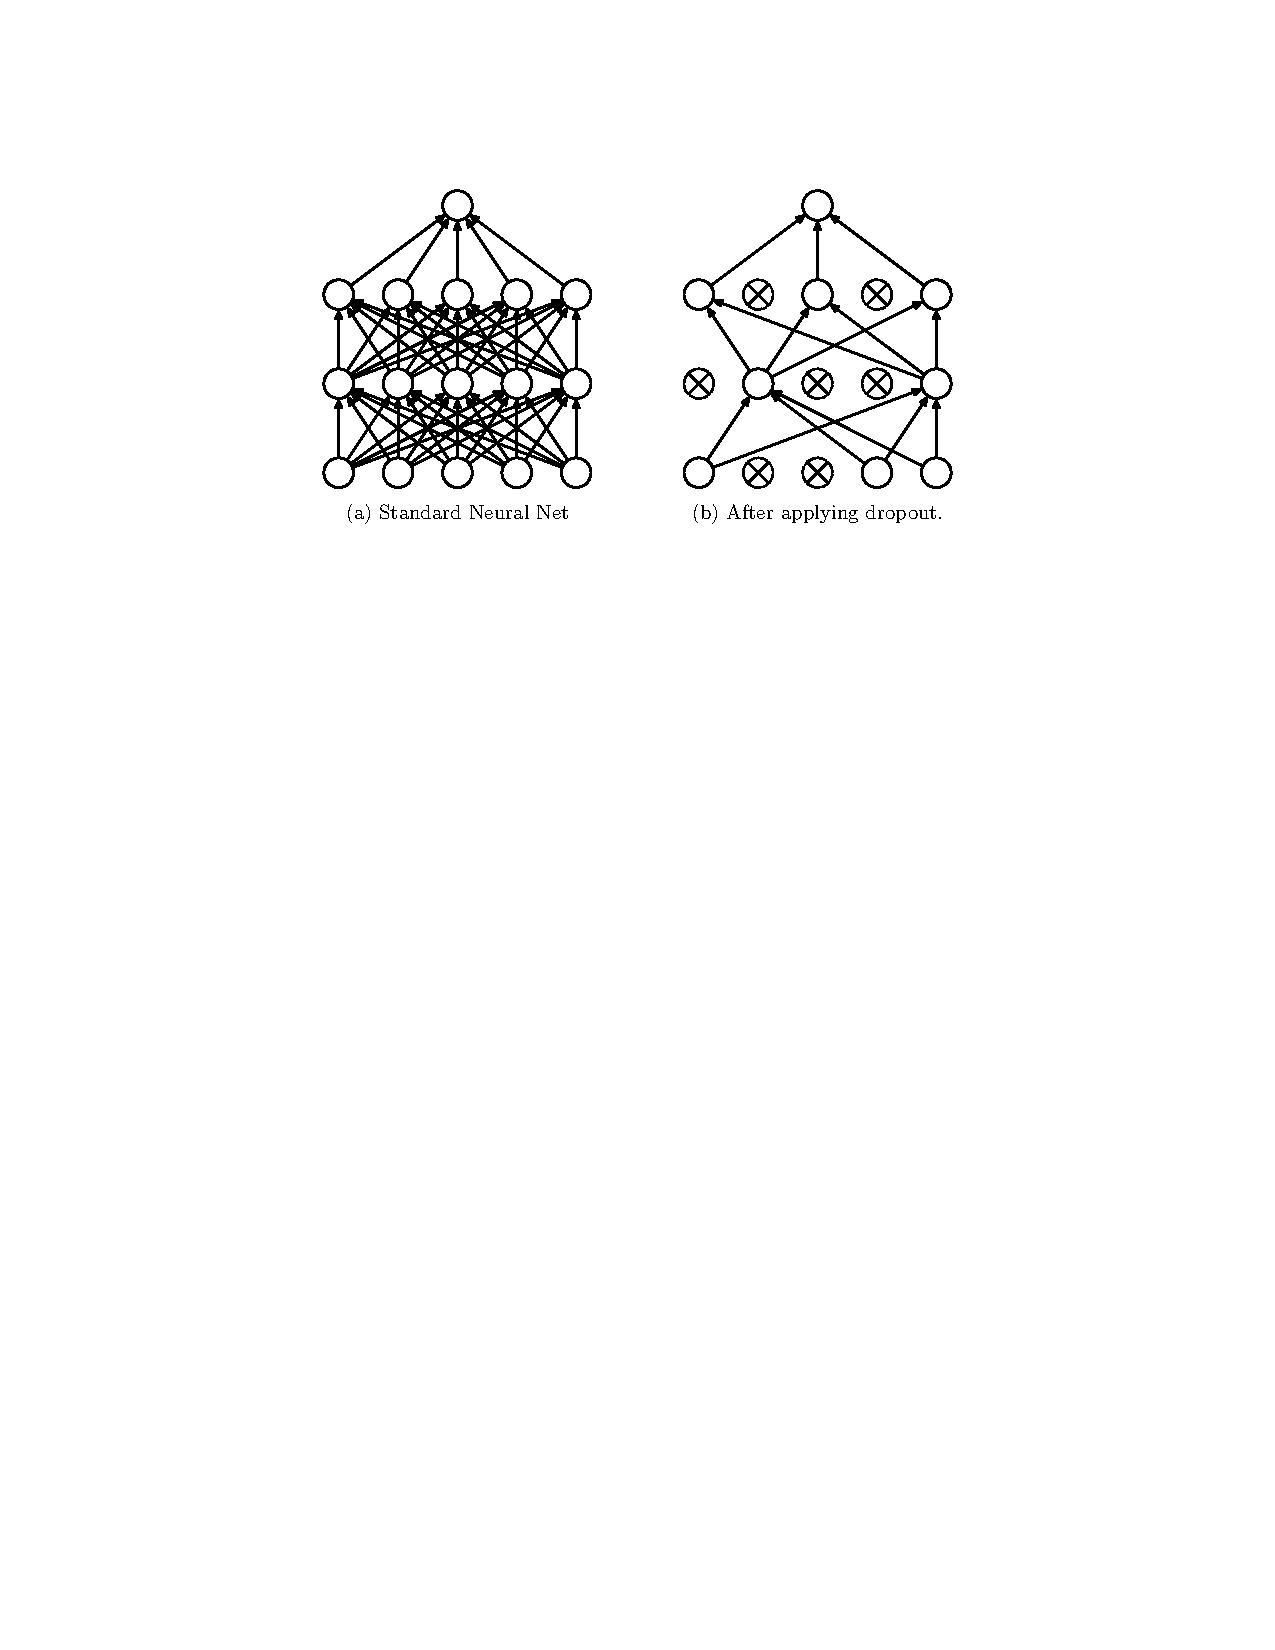
\includegraphics[scale=0.7]{Figures/dropout.pdf}
        \caption{A nerual network structure before and after applying dropout}
        \label{dropout}
    \end{figure}

    \subsubsection{Early Stopping}
    \textbf{Early Stopping} is another normal way to prevent overfitting. 
    It makes the training stop before the it is to be overfitted by the model, which is practically useful during the training process of neural networks.


    \subsection{Stochastic Gradient Descent Variants}
    \label{sgd}
    In both Gradient Descent (GD) and Stochastic Gradient Descent (SGD) parameters are updated according to an update rule to minimize a loss function in an iterative manner. Computing the exact gradient using GD in large datasets is expensive (GD is deterministic), as this method runs through all training samples to perform a single update for one iteration step. In Stochastic Gradient Descent (or on-line Gradient Descent) an approximation of the true gradient is computed. This is done by using only one or a subset of training samples for a parameter update. When using a subset of training samples, this method is called mini-batch SGD. \\

    SGD is a method to minize the loss function \(L(\theta)\)  parametrized by $\theta$. This is achieved by updating $\theta$ in the negative gradient direction of the loss function $\nabla_{\theta}L(\theta)$ with respect to the parameters, in order to decrease the loss function value. The learning rate $\eta$ determins the step size to get to the local or global minumum. 
    \begin{equation}
        \theta_{n+1} = \theta_{n} - \eta \nabla_{\theta_{n}}L(f_{\theta_{n}}(x_i), y_i)
    \end{equation}

    \subsubsection{Mini-batch Stochatic Gradient Descent}
    This method performs an update for every mini-batch of n training samples. Mini-batch SGD reduces the variance of the parameter updates. Larger mini-batches reduce the variance of SGD updates by taking the average of the gradients in the mini batch. This allows taking bigger step sizes. In the limit, if each batch contains one training sample, it is the same as regular SGD.

    \subsubsection{Distributed SGD}
    In parallel computing environments, disturbed SGD is commonly applied for optimization. For a specific architecture, basically no difference in parameter values exists when training with different computers. The parameter space can thus be further explored, and improved performance will be obtained resultantly \cite{zhang2015deep}.

    \subsection{Learning Rate Scheduling in Gradient Optimization}
    \label{learning}
    There are serval variants of SGD available. Determining the appropriate learning rate, or step size, often is a complex problem. Applying too high learning rate cause suboptimal performance, while too low learning rate led to slow convergence. Learning rate scheduling is used as an extension of the SGD algorithm to improve performance. In learning rate scheduling, the learning rate is a decreasing function of the iteration number. Therefore, the first iterations have larger learning rate and consequently cause bigger parameter changes. Later iterations have similar learning rates, responsible for fine-tuning. I gave an overview of some gradient descent optimization algorithms,

    \subsubsection{Momentum}
    Momentum method is a method to speed up the SGD in the relevant direction.  A fraction $\gamma$ of the previous update is added to the current update. The mathematical details are defined in Equation \ref{mo}.
    \begin{equation}
        \begin{aligned}
            & v_n = \gamma v_{n-1} + \eta \nabla_{\theta}L(\theta) \\
            & \theta= \theta - v_{n}
        \end{aligned}
        \label{mo}
    \end{equation} 

    \subsubsection{Nesterov Accelerated Gradient}
    The Momentum method does not take into the direction it is going in, while parameters’ next position can be approximated via the Nesterov Accelerated Gradient method. The update rule is given in Equation \ref{nag}.

    \begin{equation}
        \begin{aligned}
            & v_n = \gamma v_{n-1} + \eta \nabla_{\theta}L(\theta - \gamma v_{n-1}) \\
            & \theta= \theta - v_{n}
        \end{aligned}
        \label{nag}
    \end{equation}

    \subsubsection{Adam}
    The Adaptive Moment Estimation (Adam) optimizer \cite{DBLP:journals/corr/KingmaB14} determines an adaptive learning rate for each parameter. Apart from the decaying average for past squared gradients $v_n$, an exponentially decaying average is also maintained by Adam for the past gradients $m_n$. Estimates for the mean and the uncentered variance of the gradients are Vectors $v_n$ and $m_n$, respectively, and both of them aree biased towards zero. Bias-corrected estimates $\hat{v}_t$ and $\hat{m}_t$ are computed for the update rule in Equation \ref{adam}.

    \begin{equation}
        \theta_{n+1} = \theta_{n} - \frac{\eta}{\sqrt{\hat{v}_n} + \epsilon}\cdot \hat{m}_n
    \end{equation}

    \subsection{Backpropagation}
     The CNN requires to adjust and update its kernel parameters, or weights, for the given training data. Backpropagation\cite{werbos1990backpropagation} is an efficient method for computing gradients required to perform gradient-based optimization of the weights in neural networks [19]. Minimizing the loss function (or error function), the weights are combined together on purpose for solving the problem of optimization. Herein, the gradient of error functions need computing during each iteration, which requires continuity and differentiability of the loss functions for all iteration steps.\\

    The initial weights of an untrained CNN are randomly chosen. Consequently before training, the neural network cannot make meaningful predictions for network input, as there is no relation between an image and the its labeled output yet. By exposing the network to a training data set, comprising images and their labeled outputs with correct classes, the weights are adjusted. Training is the adaptation of the weights in such way that the difference between desired output and network output is minimized, which means that the network is trained to find the right features required for classification. There are two computational phases in a neural network, the forward pass and the backward pass in which the weights are adapted.

    \subsubsection{Forward pass}
    An image is fed into a network. The first network layer outputs an activation map. Then, this activation map is the input to the first hidden layer, which computes another activation map. Using the values of this activation map as inputs to the second hidden layer, again another activation map is computed. Carrying out this process for every layer will eventually yield the network output.

    \subsubsection{Backward pass}
    In this phase the weights are updated by backpropagation. One epoch of backpropagation consists of multiple parts, usually multiple epochs are carried out for a training image:
    \begin{enumerate}
        \item \textbf{Loss Function} In forward pass, the inputs and desired outputs are presented. A pre-defined loss function $L$ is used to minimize the disparity when comparing the input and desired output. The goal is to adjust the weights so that the loss function value decreases, this is achieved by calculating the derivative with respect to the weights of the loss function.
        \item \textbf{Backward pass} During the backward pass, the weights that have contributed the most to the loss are chosen in order to adjust them so that the total loss decreases.
        \item \textbf{Weight update} In the final part all weights are updated in the negative direction of the loss function gradient.
    \end{enumerate}
    
    Hence, gradient computation for loss functions in terms the network weights is actually the core of backpropagation problem. Computing the partial derivative $\frac{\partial L}{\partial \omega}$ is essential (carried out in the backward pass) to minimize the loss function value. Stochastic Gradient Descent (SGD) is the most common way to optimize neural networks.

    \subsubsection{Backpropagation Example for a Multi-Layer Network}
    I describe the details of backpropagation algorithm for one simple example in Figure \ref{bp}. The cost function $L$ is given below, $el$ is the error between the true output $d_l$ and network output $y_l$. The network output $y_l$ is computed in the forward pass and depends on outputs of the previous layer $v_j$ and the output layer weights $w^{o}_j$.
    \begin{figure}[!h]
        \centering
        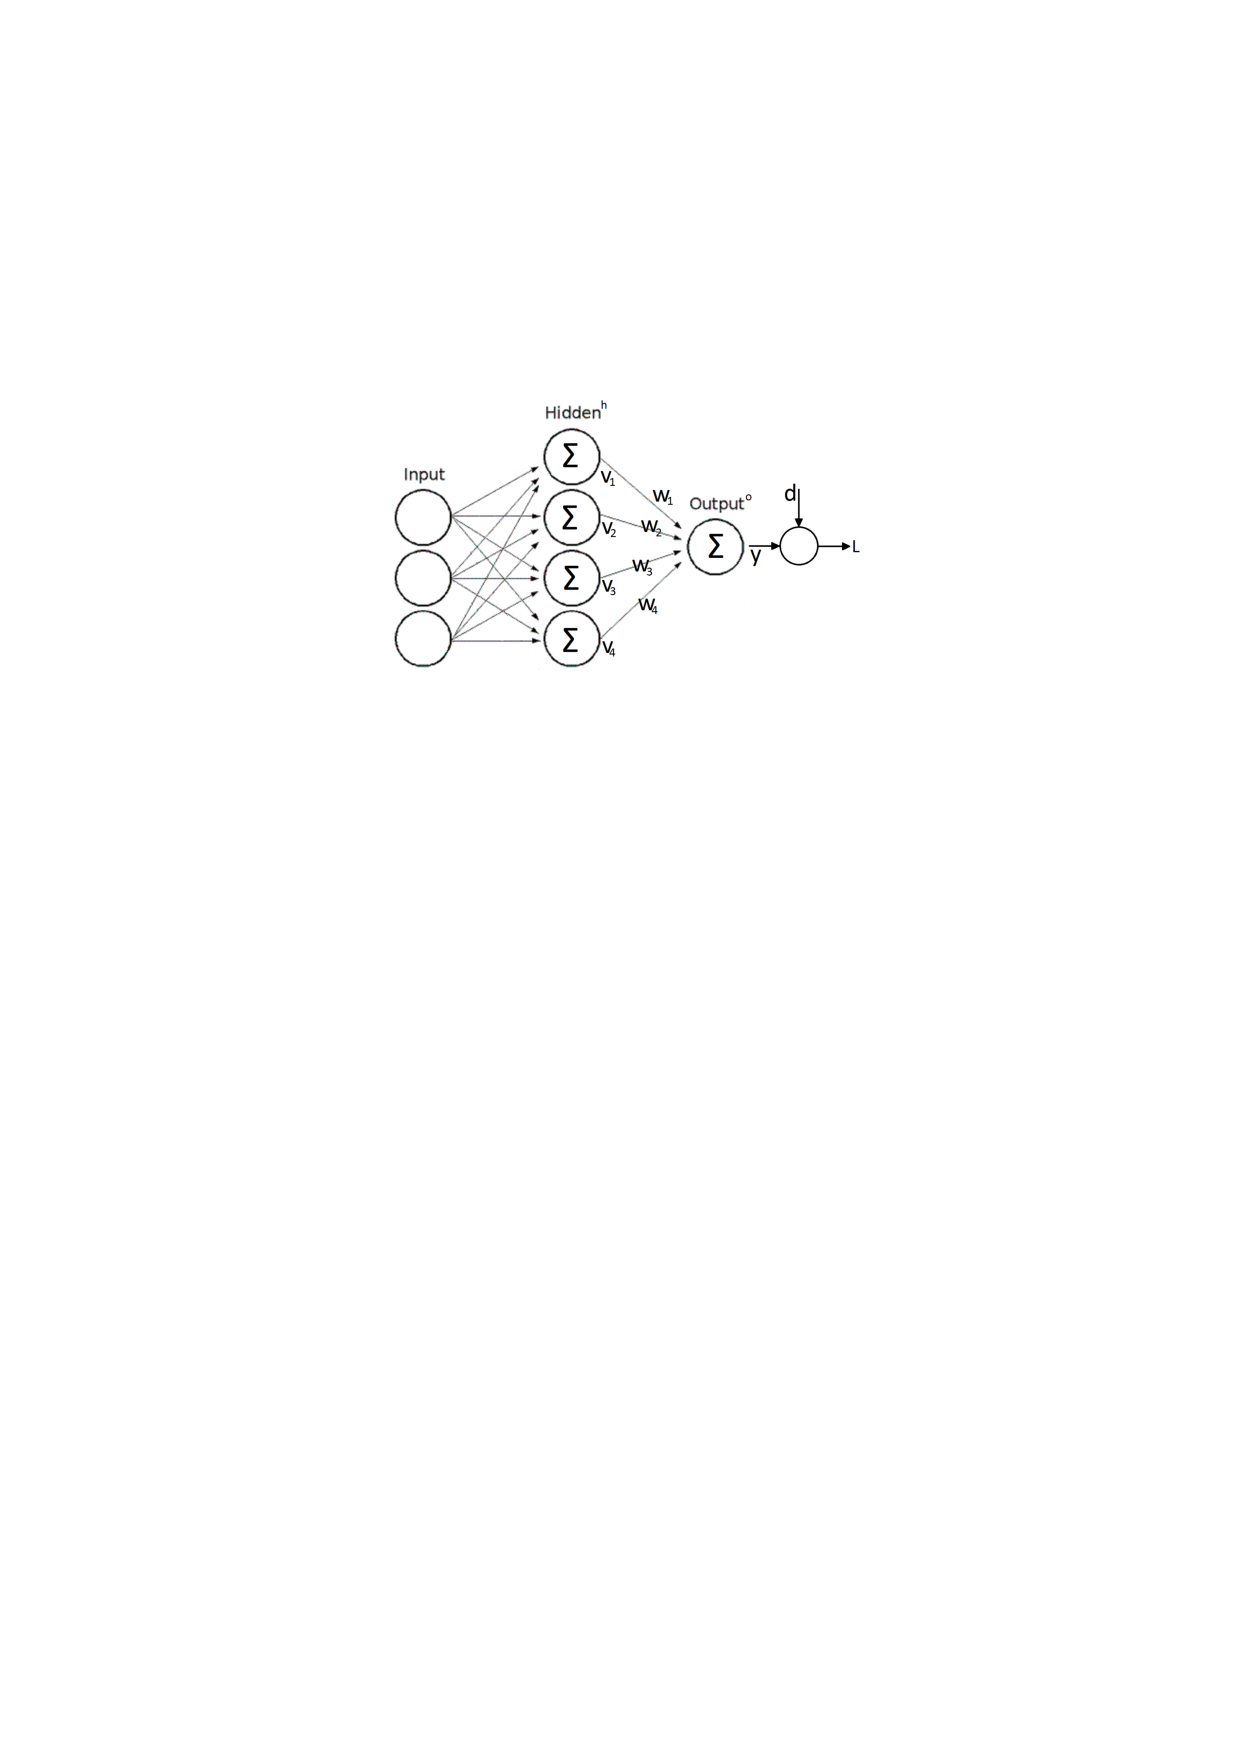
\includegraphics{Figures/bp.pdf}
        \caption{The example for showing the details of backpropagation}
        \label{bp}
    \end{figure}
    Some mathesmatical equations we can get:
    \begin{equation}
        \begin{aligned}
            L &= \frac{1}{2} \sum_{l}(e_l)^2 \\
            e_l &= d_l -y_l \\
            y_l &= \sum_{j}w^{o}_j v_j 
        \end{aligned}
        \label{me}
    \end{equation}

    The Jacobian is given by:
    \begin{equation}
        \frac{\partial L}{\partial w_{j}} = \frac{\partial L}{\partial e_l} \cdot \frac{\partial e_l}{\partial y_l} \cdot \frac{\partial y_l}{\partial w_{j}}
        \label{par_w}
    \end{equation}
    Then combining Equation \ref{me} and \ref{par_w}, we can caculate that,
    \begin{equation}
        \frac{\partial L}{\partial w^{o}_{j}} = -v_j e_l
    \end{equation}

    Using SGD updating rules \textbf{Momentum} mentioned in section \ref{sgd} Equation \ref{mo}, the output weights are updated using:
    \begin{equation}
        w^{o}_{j}(n+1) = w^{o}_{j}(n) + \alpha(n)v_j e_j
    \end{equation}
    $\alpha(n)$ stands for the learning rate in $n$th-iteration, you can see more details in section \ref{sgd}.

    After having updated the output weights, the weights in the hidden layers can be updated. As it is a backward pass, first gradients of the output layers are computed, then the gradients of the hidden layers. The Jacobian is given as follows:

    \begin{equation}
        \frac{\partial L}{\partial w^{h}_{ij}} = \frac{\partial L}{\partial e_l} \cdot \frac{\partial e_l}{\partial y_l} \cdot \frac{\partial y_l}{\partial v_{j}} \cdot \frac{\partial v_j}{\partial w^{h}_{ij}}
        \label{par_w}
    \end{equation}

    Based on the networks shown in Figure \ref{bp}, we can define $v_j$ based on $w_ij$ and input $x_i$
    \begin{equation}
        v_j = \sum_{i=1}^{N_{input}}x_i\cdot w^{h}_{ij}
        \label{vj}
    \end{equation}


    Then combining Equation \ref{par_w} and \ref{vj}, we can calculate the Jacbian,
    \begin{equation}
        \frac{\partial L}{\partial w_{ij}^{h}} = -e_l w_j^{o} x_i
    \end{equation} 

    Which yields the update rule for the hidden layers:
    \begin{equation}
        w_{ij}^{h}(n+1) = w_{ij}^{h}(n)+ \alpha(n)e_l w_j^{o} x_i
    \end{equation}
    Finally the network is tested using a test dataset, this dataset contains data that differ from the ones in the training dataset. By increasing the amount of training data, the more training iterations are carried out, the better the weights are tuned.
